\chapter{Lecture 29 - Solving Boundary Value Problems, MATLAB Built-in Methods}
\label{ch:lec29n}
\section{Objectives}
The objectives of this lecture are to:
\begin{itemize}
\item Introduce MATLAB built-in functions \lstinline[style=myMatlab]{bvp4c} and \lstinline[style=myMatlab]{bvp5c} and show how to use them.
\item Do an example problem.
\end{itemize}
\setcounter{lstannotation}{0}

\section{BVP4C and BVP5C}

Both of these built-in solvers use variations of the finite difference method.  For this lecture, we will \emph{not} delve into any of the inner working details of the functions.  Rather, I will seek only to show you how to \emph{use} the functions.  The interface for both functions are the same so, for all intents and purposes relevant for this class, you can use them interchangeably.  This is not to say that the differences between the two functions are trivial.  Interested readers are advised to consult the MATLAB documentation to learn more.

\newthought{To get a solution} to a BVP using \lstinline[style=myMatlab]{bvp4c} or \lstinline[style=myMatlab]{bvp5c}, the user has to provide the typical information:
\begin{enumerate}
\item \emph{The governing equation.} As with other built-in ODE solvers, this is provided as a function that returns the value for:
\begin{equation*}
\frac{dw}{dx} = f(x,w)
\end{equation*}
where here we indicate the dependent variable with $w$.  Since the BVPs of interest to us are 2\textsuperscript{nd}-order and higher, the dependent variable $w$ will be a vector and the governing equation for an $n$\textsuperscript{th}-order BVP will be a system with $n$ equations.  In the examples presented here, this function will ordinarily be implemented as a local function.  For particularly simple governing equations, an inline ``anonymous'' function may be used.
\begin{lstlisting}[style=myMatlab]
function dw = fun(x,w)
.
. % governing equation implemented here %
.
end
\end{lstlisting}

\item \emph{Boundary conditions}.  Recall with IVP solvers like \lstinline[style=myMatlab]{ode45} or \lstinline[style=myMatlab]{ode78} initial conditions were simply given as vectors.\sidenote{This reflects the difference in what types of conditions are given for IVPs compared to BVPs.  For IVPs, the only option presented for initial conditions was to make a direct assignment to the dependent variable and its derivative at one end of the domain.}  This is roughly equivalent to having only type 1 and type 2 boundary conditions.  In order to gain the expressiveness that we need, a different approach is taken for BVP solvers.  We provide a \emph{residual function} that accepts as arguments the dependent variable and its derivatives at each boundary; the function returns the boundary condition in \emph{residual} form.\sidenote{By \emph{residual form} we just mean that the boundary condition is used as it is stated but with all of the terms moved to the left-hand-side of the equation.}  Using the example from Lecture 28 where the boundary conditions were:
\begin{equation*}
T(0) = T_A, \ \ T(0.1) = T_B
\end{equation*}
we could encode these as follows:
\begin{lstlisting}[style=myMatlab]
bcfun = @(wa,wb) [wa(1) - Ta; wb(1) - Tb];
\end{lstlisting}
where \lstinline[style=myMatlab]{wa(1)-Ta} is equivalent to $T(0)-T_A$; and \lstinline[style=myMatlab]{wb(1)-Tb} is equivalent to $T(0.1)-T_B$.\sidenote{If I need to refer to the derivative of the dependent variable at either boundary, I would refer to them as \lstinline[style=myMatlab]{wa(2)} or \lstinline[style=myMatlab]{wb(2)}, respectively.}

\item \emph{Initial mesh and solution guess.} Like other built-in MATLAB functions for solving ODEs, \lstinline[style=myMatlab]{bvp5c} will adapt the mesh as needed to provide a solution that satisfies the specified error tolerances.\sidenote{As with other solvers, absolute and relative error tolerances are provided by default and can be changed by the user as desired.} To specify the mesh and initial solution guess, we use the built-in function \lstinline[style=myMatlab]{bvpinit} as shown in the listing below:
\begin{lstlisting}[style=myMatlab]
a = 0; b = 1; % domain 0 < x < 1
Yguess = [1 0]; % guess constant solution
initial_mesh = [a b]; % as coarse as possible /*!\annotation{lst:ann29n-1}!*/
solinit = bvpinit(initial_mesh,Yguess);
\end{lstlisting}
\marginnote[-0.8cm]{

\noindent \ref{lst:ann29n-1} \lstinline[style=myMatlab]{bvp5c} will adapt this mesh as needed.  Note that the final mesh will not generally be uniform.
}
Alternatively, you may specify a more refined initial mesh using a tool like \lstinline[style=myMatlab]{linspace}. 
\marginnote{

\vspace{0.85cm}

\noindent \ref{lst:ann29n-2} I have yet to encounter a BVP where it was necessary to provide an initial solution guess more detailed than a constant value.

}
\begin{lstlisting}[style=myMatlab]
a = 0; b = 1; N = 100;
Yguess = [1 0];/*!\annotation{lst:ann29n-2}!*/
initial_mesh = linspace(a,b,N);
solinit = bvpinit(initial_mesh,Yguess);
\end{lstlisting}

\item \emph{Provide any options.}  Default values are provided for all needed options.  Any named parameter can be set using the built-in function \lstinline[style=myMatlab]{bvpset(name1,value1,name2,value2,...)}.  An example is shown in the listing below.
\begin{lstlisting}[style=myMatlab]
options = bvpset('RelTol',1e-3,'AbsTol',1e-6,'NMax',1000);
\end{lstlisting} 

\end{enumerate}

\newthought{The syntax for} a typical call to \lstinline[style=myMatlab]{bvp5c} is shown in the listing below:
\begin{lstlisting}[style=myMatlab]
sol = bvp5c(fun,bcfun,solinit,options);
\end{lstlisting}
The return value \lstinline[style=myMatlab]{sol} is a structure that contains, among other information, fields for the solution, \lstinline[style=myMatlab]{sol.y}, at discrete grid points, \lstinline[style=myMatlab]{sol.x}.\sidenote{Once again, the reader is encouraged to review the MATLAB documentation to learn what other useful information is packed into the other fields of the output solution structure.}

\subsection{Example \#1}

\noindent Consider the following boundary value problem:
\begin{table}
\begin{tabular}{l l}
Governing Equation: & $\frac{d^2y}{dx^2}-y=sin(x), \ \ 0 < x < 2$ \\
BCs: & $y(0) = 1, \ \ y(2) = 0$ \\
\end{tabular}
\end{table}

\vspace{0.25cm}

\noindent Using basic techniques you can show that the general solution to the governing equation is:
\marginnote{This is a 2\textsuperscript{nd}-order, linear, constant-coefficient, non-homogeneous ordinary differential equation.  See Lecture 5 in the analytical methods portion of this text for a review on how to solve problems like this.}
\begin{equation*}
y(x) = c_1\sinh{(x)} + c_2\cosh{(x)}-\frac{1}{2}\sin{(x)}
\end{equation*}
Applying the boundary conditions we get the following values for the remaining constants:
\begin{align*}
c_1 &= \frac{\frac{1}{2}\sin{(2)}-\cosh{(2)}}{\sinh{(2)}} \\
c_2 &= 1
\end{align*}
Let us use MATLAB and \lstinline[style=myMatlab]{bvp5c} to solve this BVP numerically.\marginnote{\textbf{Note:} It is always a good idea, when learning to use new tools, to use the tool on a problem for which you already know the correct answer.}
\setcounter{lstannotation}{0} % reset the counter.
\marginnote[3.0cm]{

\noindent\ref{lst:ann29n-ex1-1} This is one of the simple cases where the governing equation can easily be implemented with an in-line function.

\vspace{2.0cm}

\noindent\ref{lst:ann29n-ex1-2} The output solution structure, \lstinline[style=myMatlab]{sol5c}, also has a field containing the maximum residual error in the field: \lstinline[style=myMatlab]{sol5c.stats.maxerr}

}
\begin{lstlisting}[style=myMatlab,name=lec29n-ex1]
clear
clc
close 'all'
%% Construct Exact Solution
C1 = (0.5*sin(2)-cosh(2))/sinh(2);
C2 = 1;
y_exact = @(x) C1*sinh(x) + C2*cosh(x) - 0.5*sin(x);

%% Solve with BVP5C
Ya = 1; Yb = 0;
xMin = 0; xMax = 2;
Yguess = [1 0];
F = @(x,w) [w(2); w(1)+sin(x)]; /*!\annotation{lst:ann29n-ex1-1}!*/
bcfun = @(ya,yb) [ya(1)- Ya; yb(1)-Yb];
solinit = bvpinit([xMin xMax],Yguess);
options = bvpset('RelTol',1e-10,'AbsTol',1e-8,'NMax',5000);
sol5c = bvp5c(F,bcfun,solinit,options);

%% Calculate the Relative Error
rel_err = norm(y_exact(sol5c.x)-sol5c.y(1,:),2)/...
    norm(y_exact(sol5c.x),2);          /*!\annotation{lst:ann29n-ex1-2}!*/
fprintf('Relative error = %g \n',rel_err);
\end{lstlisting}
\begin{lstlisting}[style=myMatlab,name=lec29n-ex1]
%% Plot the solution
plot(sol5c.x,sol5c.y(1,:),'-sb','linewidth',3);
title('Solution with BVP5C','fontsize',14,...
    'fontweight','bold');
xlabel('X','fontsize',12,'fontweight','bold');
ylabel('Y(X)','fontsize',12,'fontweight','bold');
grid on
\end{lstlisting}


\noindent A plot of the solution is shown in Figure \ref{fig:lec29n-ex1-bvp5c-sol}. The initial maximally coarse grid has been refined adaptively to arrive at a solution that satisfies the user-specified relative error tolerance.  

\begin{marginfigure}[-3.5cm]
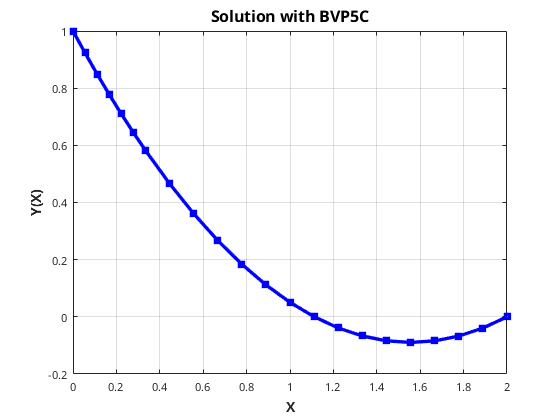
\includegraphics{lec29n-ex1-bvp5c-sol.png}
\caption{Solution of example problem with \lstinline[style=myMatlab]{bvp5c}.}
\label{fig:lec29n-ex1-bvp5c-sol}
\end{marginfigure}

\subsection{Example \#2}

\noindent The axial temperature variation of a current-carrying bare wire, as illustrated in Figure \ref{fig:lec29n-ex2-schematic}, is described by the following boundary value problem:

\begin{marginfigure}
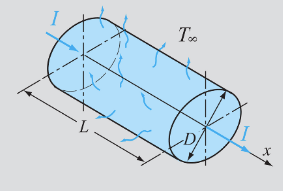
\includegraphics{lec29n-ex2-schematic.png}
\caption{Current-carrying wire schematic.}
\label{fig:lec29n-ex2-schematic}
\end{marginfigure}

\begin{table}
\begin{tabular}{l l}
ODE: & $\frac{d^2T}{dx^2}-\frac{4h}{kD}\left(T-T_{\infty}\right)-\frac{4\epsilon \sigma_{\text{SB}} \left(T^4 - T_{\infty}^4 \right)}{kD}=-\frac{I^2\rho_e}{k \left(\frac{1}{4}\pi D^{2}\right)^2} $\\
BCs: & $T(x=0)=300K, \ \ \frac{dT}{dx}\Bigl|_{x=\sfrac{L}{2}}=0$ \\
\end{tabular}
\end{table}
\marginnote[0.5cm]{\textbf{Note:} This is a 2\textsuperscript{nd}-order, non-linear, non-homogeneous boundary value problem.  This author is not aware of any analytic technique that would work to find an exact solution.  Nonetheless, we will be able to solve this problem using \lstinline[style=myMatlab]{bvp5c} with not much more effort than what was required for the last example; the difference lies mainly in implementing the governing equation.}
\noindent where $T$ is the temperature in Kelvin, $x$ is the coordinate along the wire, $k = 72 \text{W/m-K}$ is the thermal conductivity, $h=2000 \text{W/m}^2\text{-K}$ is the convective heat transfer coefficient, $\epsilon=0.1$ is the radiative emissivity, $\sigma_{\text{SB}}=5.67\times 10^{-8} \text{W/m}^2\text{-K}^4$ is the Stefan-Boltzmann constant, $I=2$ amps is the current, $\rho_e=32\times 10^{-8}$ Ohm-m is the electrical resistivity, $T_{\infty}=300$ K is the ambient temperature, $D=7.62\times 10^{-5}$m is the wire diameter, and $L=4.0\times 10^{-3}$m is the length of the wire.
\setcounter{lstannotation}{0} % reset the counter.
\marginnote{

\vspace{0.1cm}

\noindent \ref{lst:ann29n-ex2-1} For this problem it is somewhat less practical to use an in-line function to implement the governing equation.  We include \lstinline[style=myMatlab]{ex2(x,t)} as a local function.

\vspace{0.4cm}

\noindent \ref{lst:ann29n-ex2-2} Obviously we could have omitted the zero in the expression `\lstinline[style=myMatlab]{yb(2)-0}', but for the sake of clarity it is not a horrible idea to include that term.  The point of this example is to illustrate a problem with a type 2 boundary condition.

}
\begin{lstlisting}[style=myMatlab,name=lec29n-ex2]
F = @(x,t) ex2(x,t);  /*!\annotation{lst:ann29n-ex2-1}!*/
L = 4e-3; % m, length of wire
xMin = 0; xMax = L/2;
To = 300; % K, temperature at x=0

bcfun = @(ya,yb) [ya(1)- To; yb(2) - 0]; /*!\annotation{lst:ann29n-ex2-2}!*/
Tguess = [To 0]; % second entry is dT/dx
solinit = bvpinit([xMin xMax],Tguess);
options = bvpset('RelTol',1e-10,'AbsTol',1e-8,'NMax',5000);
sol2 = bvp5c(F,bcfun,solinit,options);

figure(1)
plot(sol2.x,sol2.y(1,:),'-sb','linewidth',3);
grid on
title('Example 2 Solution','fontsize',16,...
    'fontweight','bold');
xlabel('X [m]','fontsize',14,'fontweight','bold');
ylabel('T(X) [K]','fontsize',14,'fontweight','bold');
set(gca,'fontsize',12,'fontweight','bold');
\end{lstlisting}

\noindent The solution is shown in Figure \ref{fig:lec29n-ex2-sol}.  The local function used to implement the governing equation is shown in the next listing.
\begin{marginfigure}
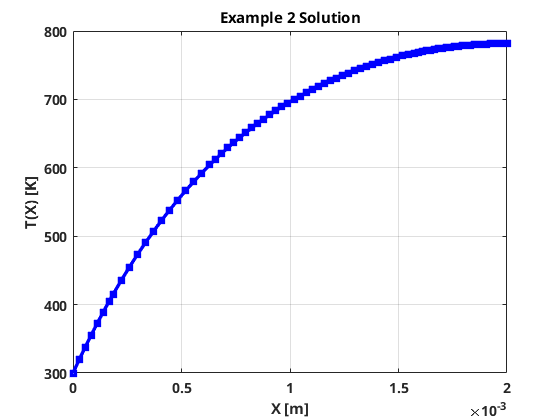
\includegraphics{lec29n-ex2-sol.png}
\caption{Solution for Example \#2.}
\label{fig:lec29n-ex2-sol}
\end{marginfigure}

\begin{lstlisting}[style=myMatlab,name=lec29n-ex2]
%% Local Functions
function dTdx = ex2(~,T) /*!\annotation{lst:ann29n-ex2-3}!*/
k = 72; % W/m-K
h = 2000; % W/m^2-K
emiss = 0.1;
sigma_sb = 5.67e-8; % W/(m^2-K^4)
I = 2; % amps
rho_e = 32e-8; % Ohm-m
Tinf = 300; % K
D = 7.62e-5; % m

% make some terms to simplify the equation
c1 = 4*h/(k*D);
c2 = 4*emiss*sigma_sb/(k*D);
c3 = -I^2*rho_e/(k*(0.25*pi*D^2)^2);
dTdx = [T(2);
    c1*(T(1) - Tinf) + c2*(T(1).^4 - Tinf^4) + c3];
end
\end{lstlisting}

\marginnote[-6.0cm]{

\noindent \ref{lst:ann29n-ex2-3} Reminder that, since the governing equation is not a function of the independent variable---it is \emph{autonomous}, in the language of ODEs---we can (and should) use a tilde to take the place of the first argument of the function.
}

